


\begin{abstract}
Hypergraph implementations have modeled real life systems with material gains in performance over graph representations of the same problems. Odometers serve as an alternative representation of hyperedges in a hypergraph from the traditional incident matrix. The traversal of hyperedges in a hypergraph using an odometer and incrementing function is shown to be similar to traversing a Hilbert curve through a $N^\infty$ dimensional Hilbert space.
\end{abstract}

\section{Introduction}
Hypergraphs are composed of a set of vertexes and hyperedges $HG = (v, he)$ commonly denoted in matrix format show below. Each column represents a node’s set of hyperedges. Each row represents a set of nodes in a hyperedge. The sample hypergraph presented as both nodes linked by hyperedges and hyperedges linked by nodes in the subsequent pictures. Displaying high dimensionality objects such as hypergraphs is a complex problem with active ongoing research in the area..
\begin{center}
\begin{tabular}{l | c | r}

\begin{tabular}{l l l l l l l l}
			 & $V_1$ & $V_2$ & $V_3$ & $V_4$ & $V_5$ & $V_6$ \\
$E_1$  &     1 		& 1          & 1 			& 0 			& 0 			& 0 		 \\
$E_2$  &     0 		& 1          & 1 			& 0 			& 0 			& 0 		 \\
$E_3$  &     0 		& 0          & 1 			& 0 			& 1 			& 1 		 \\
$E_4$  &     0 		& 0          & 1 			& 1			& 0 			& 0 		 \\
$E_5$  &     1 		& 0          & 0 			& 1			& 0 			& 1 		 \\
\end{tabular}

& 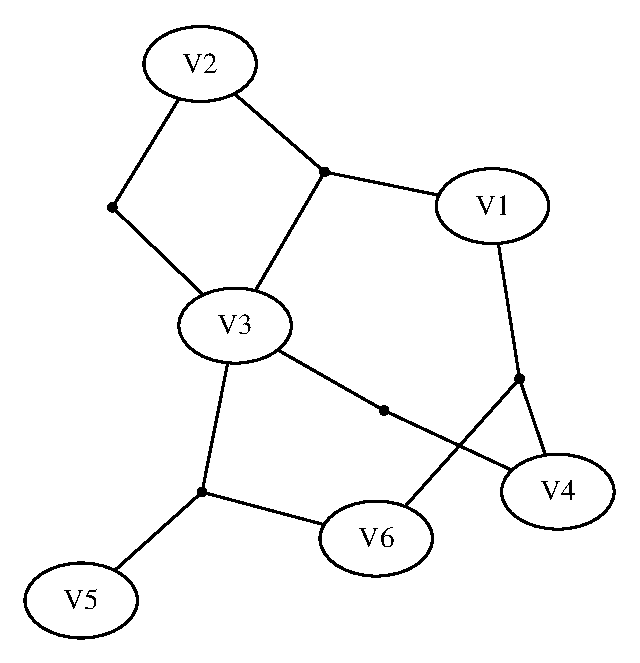
\includegraphics[scale=.25]{vertex_graph.eps} & 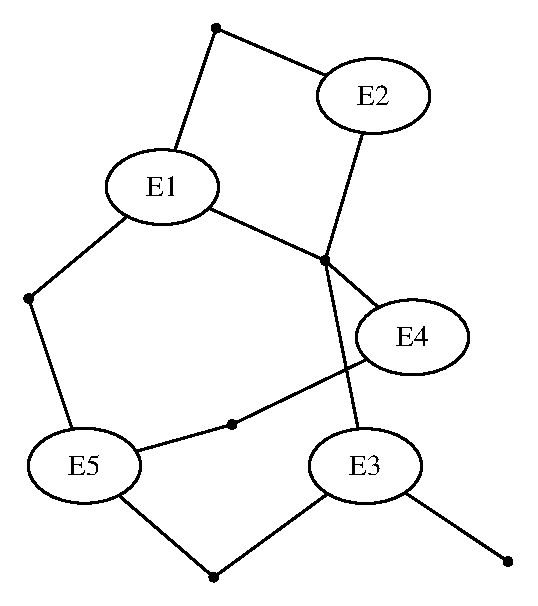
\includegraphics[scale=.25]{edge_graph.eps}\
\end{tabular}
\end{center}


\newpage

\section{Hypergraph, odometer \& hyperedges:}

\begin{lstlisting}
def makeHyperGraph(hyperedge):
    vector_things = [0 for x in range(len(hyperedge))]
    address_lookup = dict()
    for i in range(len(hyperedge)):
        node = hyperedge[i]
        vector_things[i] = node
        address_lookup[node] = i
    return (vector_things,address_lookup)

def getHyperEdge(hypernet,odometer):
    (vector_things,address_lookup) = hypernet
    hyperedge = [0 for x in range(len(odometer))]
    space_size = len(vector_things)
    for index in range(len(odometer)):
        node_index = odometer[index] % space_size
        hyperedge[index] = vector_things[node_index]
    return hyperedge
    
def getOdometer(hypergraph,hyperedge):
    (vector_things,address_lookup) = hypergraph
    odometer = [0 for x in range(len(hyperedge))]
    for index in range(len(hyperedge)):
        node = hyperedge[index]
        odometer[index] = address_lookup[node]
    return odometer
\end{lstlisting}
\newpage
\begin{wrapfigure}{r}{0.5\textwidth}
  \begin{center}
    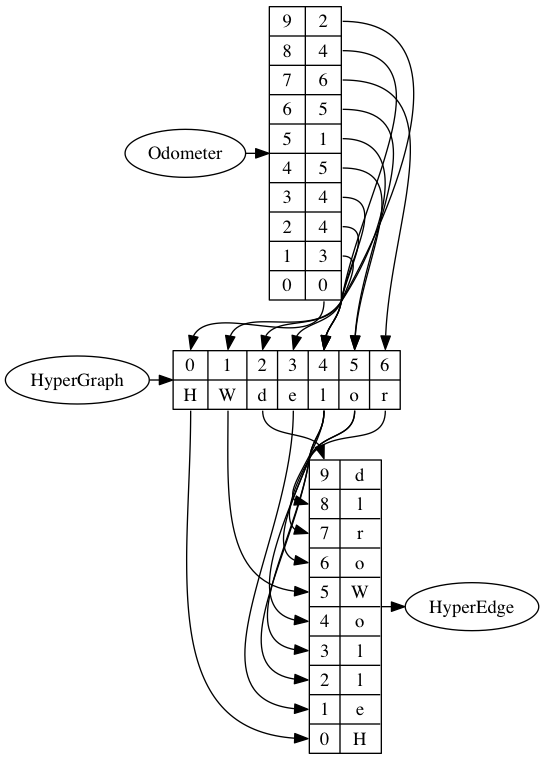
\includegraphics[width=0.48\textwidth]{odometers.png}
  \end{center}
\end{wrapfigure}

%\centering
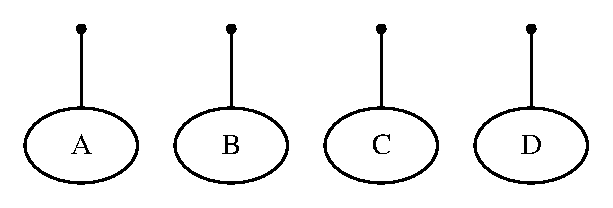
\includegraphics[width=0.44\textwidth]{List.eps}
%\caption{\label{fig:frog1}Hyperedge collection as list}
\section{Concepts}

\indent The presented hypergraph model supports conversion from an odometer to hyperedge or hyperedge to odometer in one function call. Traditionally all hyperedges in a hypergraph are explicitly declared and stored in memory or disk. \\

This model can explore super dense hypergraphs: $2^N$, $N^N$ even $N^M$ hyperedges that standard matrix hypergraph models cannot represent. These hypergraphs share the common characteristic that they must be explored algorithmically. This image demonstrates a single odometer to hyperedge conversion via arbitrary hypergraph using the given definitions.\\

\begin{lstlisting}
hypergraph =makeHyperGraph(sorted(set("Hello World!")))

odometer = getOdometer(hypergraph, "Hello World!")

hyperedge = getHyperEdge(hypergraph,odometer)

(vector_of_things,address_lookup) = hypergraph
\end{lstlisting}
